%\documentclass[final,5p,twocolumn,10pt,number]{elsarticle}\usepackage{amsmath}\usepackage{pxfonts,amssymb}

\documentclass[review,3p,times,12pt,number]{elsarticle}\usepackage{amsmath}\usepackage{amssymb}






\usepackage{multicol,enumitem,multirow,booktabs}


\newlength{\smalltable}
\setlength{\smalltable}{252pt}


\newtheorem{proposition}{Proposition}
\newtheorem{definition}{Definition}


\usepackage[vlined,ruled,linesnumbered]{algorithm2e}
\SetKwComment{tcp}{/\!/\,}{}
\SetArgSty{textrm}
\SetKwProg{Procedure}{procedure}{}{end~procedure}
\SetKwProg{Function}{function}{}{end~function}
\SetKwFor{Repeat}{repeat}{times do}{end~loop}
\SetKwFunction{Move}{Move}
\SetKwFunction{Relocate}{Relocate}
\SetKwFunction{EvalMove}{EvalMove}
\SetKwFunction{Valid}{ValidTasks}
\SetKwFunction{Largest}{LargestPriorityTasks}
\SetKwFunction{EvalTask}{EvalTask}
\SetKwFunction{MoveNeed}{MoveNeed}
\SetKwFunction{Fill}{Fill}
\SetKwFunction{BiReceiver}{BiReceiver}
\SetKwFunction{BiSender}{BiSender}
\SetKwFunction{Interim}{Interim}
\SetKwFunction{InterimFull}{InterimFull}
\SetKw{Break}{break~while}

\renewcommand{\citet}[1]{\citeauthor{#1}~\citep{#1}}
\makeatletter
\def\NAT@def@citea{\def\@citea{\NAT@separator}}
\makeatother


\usepackage[colorlinks=true]{hyperref}
%\AtBeginDocument
{
\hypersetup{linkcolor =magenta,
anchorcolor =red,
citecolor =cyan,
filecolor =red,
menucolor =red,
runcolor =red,
urlcolor =cyan
}
}


\usepackage{caption}
\captionsetup[figure]{font=small}
\captionsetup[table]{skip=0.5ex,font=small}



\renewcommand{\gets}{\coloneqq}
\renewcommand{\emph}[1]{\textbf{\textit{#1}}}



\newcommand{\mss}{s^\mathrm{src}}
\newcommand{\mds}{s^\mathrm{dst}}
\newcommand{\mts}{s^\mathrm{tmp}}




\newcommand{\setalgo}{\linespread{1}\fontsize{10}{12}\selectfont}
\newcommand{\settab}{\linespread{1}\fontsize{10}{12}\selectfont}

\sloppy


\begin{document}

\begin{frontmatter}

\journal{EJOR}
\title{A generic feasibility-based heuristic scheme for the container pre-marshalling problem}
\author[cityu]{Bo Jin\corref{cor}}
\ead{msjinbo@cityu.edu.hk}
\author[cityu]{Andrew Lim\fnref{lim}}
\ead{alim.china@gmail.com}

\author[shu]{Ning Wang}
\ead{ningwang@shu.edu.cn}

\cortext[cor]{Corresponding author. Tel: +852 3442 5296}



\address[cityu]{Department of Management Sciences, City University of Hong Kong, Tat Chee Avenue, Kowloon Tong, Hong Kong}
%\address[andrew]{School of Physical and Mathematical Sciences, Nanyang Technological University, Singapore 637371, Singapore}
\fntext[lim]{Andrew Lim is currently on no pay leave from City University of Hong Kong.}
\address[shu]{Department of Information Management, School of Management, Shanghai University, Shanghai, China}

\begin{abstract}

This paper addresses the container pre-marshalling problem (CPMP), the problem of reorganizing containers inside a storage bay such that additional reshuffling is not needed in the subsequent retrieval process. Traditional heuristic approaches handle containers in the reverse order of future retrievals. We propose a generic feasibility-based heuristic scheme for the CPMP, which is a departure from the traditional heuristic strategy. An implementation of the heuristic scheme, the greedy and speedy heuristic, is also proposed, in which four well designed heuristic techniques are applied. Computational experiments are conducted to showcase the proposed heuristic's performance.
\end{abstract}

\begin{keyword}
container pre-marshalling problem \sep heuristic \sep logistics \sep feasibility-based heuristic scheme
\end{keyword}
\end{frontmatter}




\section{Introduction}



Since the commencement of containerization, the global use of standardized containers has dramatically improved international trade. Containers enable the smooth flow of goods between multiple transportation modes without directly handling the freight. Over the years, stringent requirements such as just-in-time operations from consignors have created additional challenges for the container transportation industry.

Container yards --- the spaces dedicated to the transshipment, handover, loading, consolidation, maintenance, and storage of containers --- are key components of maritime container terminals. Some yards act as exchange venues for container transfers between different transportation modes while others are used as caches for temporary storage or as warehouses for long-term storage.

Generally, a container yard is divided into several yard blocks, each of which consists of several parallel bays.  A bay is formed by a row of stacks. Usually the containers stored in the same bay have the same dimensions. Equipments such as rubber tyre gantry cranes, rail-mounted gantry cranes, and  reach stackers are frequently used in container yards. Figure~\ref{fig:block} illustrates an example of a yard block.

\begin{figure}[htbp]
\centering
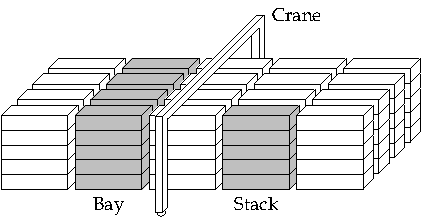
\includegraphics{figs/block.pdf}
\caption{Yard block.}
\label{fig:block}
\end{figure}

Because containers in the same stack are organized last-in-first-out, to retrieve lower containers, those on top must first be relocated. Such forced movements are known as container \emph{reshuffles}. According to recent reviews~\citep{carlo2014,lehnfeld2014}, terminals deal with three major decision problems related to container reshuffling. The first problem is the selection of storage locations for arriving containers. The second is the \emph{pre-marshalling} problem, which addresses the reorganization of containers inside a storage area such that no reshuffling is further required. The last problem  minimizes the total operational cost in the container retrieval process, measured by the number of relocations conducted or the total operational time. The  aim is to improve terminals' performance levels, including their throughput rate per berth or the turnaround time of vessels or road trucks~\citep{kim2015}.

This paper investigates the \emph{container pre-marshalling problem} (CPMP), in which the containers within a single bay are reshuffled before they are retrieved to facilitate retrieval without subsequent reshuffling. It is assumed that the retrieval order of the containers is known beforehand and that no container arrives at or leaves from the bay during pre-marshalling.

This paper makes two main contributions to the literature. First, a generic feasibility-based heuristic scheme is proposed, based on a new state feasibility concept. The heuristic scheme breaks away from the traditional heuristic strategy, greatly enriching the methodology for the CPMP\@. The second contribution is an implementation of the generic scheme, the \emph{greedy and speedy heuristic} (GASH), in which four well designed heuristic techniques are applied. The GASH performs outstandingly on both dense and loose instances, compared with existing heuristics.

The remainder of this paper is structured as follows. Section~\ref{sec:literature} reviews existing approaches in the literature. Section~\ref{sec:notation} lists the notation used throughout this paper and Section~\ref{sec:problem} gives a mathematical description of the problem. Comprehensive description of the heuristic scheme, four available techniques, and the proposed GASH can be found successively in Sections~\ref{sec:scheme}--\ref{sec:gash}. Section~\ref{sec:experiment} illustrates the results of our computational experiments, and the last section concludes this paper and identifies future research directions.

\section{Recent work}
\label{sec:literature}

To the best of our knowledge, ** works study the solutions to the pre-marshalling solutions. The study on pre-marshalling problem is few compared with other problems in ports, such as berth allocation problem and quay crane problem. One reason behind is that the pre-marshalling problem is typical, and the variants are few. Variants are TODO.

\citet{lee2007} develop an integer programming model for the CPMP\@. In this work, the problem is formulated as a multi-commodity network flow problem. The overall network is divided into several subnetworks, with each subnetwork representing an intermediate layout. The nodes in a subnetwork correspond to the slots that accommodate containers, and the commodities correspond to the containers stored in the bay. Every valid flow in the network represents a solution to the pre-marshalling problem. The model provides an innovative viewpoint to the problem, however, its performance is limited because the network is too large even for small problem instances.


\citet{cas2009} provide a greedy heuristic, the corridor method, for solving the problem. The heuristic selects the direction of movement in a randomized manner according to the attractiveness of available successors confined by the corridor. The attractiveness is measured by an estimated number of additional relocations needed for the particular successor.
A local improvement procedure is also conducted to accelerate the heuristic process.

A neighborhood search approach is proposed by \citet{lee2009}, which repeatedly modifies the current solution until some termination condition is met. Unlike the other existing solution construction approaches, the neighborhood search  is required to start from a pre-generated initial solution.
A feasible solution can be further improved by a four-step procedure, and the diversity of the neighborhood is raised by multiple subroutines. The main drawback of the approach is the unreliability of random solution modifications, i.e., the feasibility of the resulting new solutions are not always ensured.

\citet{bort2012} describe a tree search procedure for solving the problem.
In the tree search structure, solutions are constructed by compound moves  instead of single moves. Moves are classified into four types, and only the most promising ones are adopted in the branching scheme.

There are two studies in the literature regarding heuristic approaches. They adopt the same heuristic strategy that containers are handled in reverse of their retrieval order.

\citet{exp2012} provide the first container-oriented heuristic for the CPMP, named the lowest priority first heuristic (LPFH). The LPFH iteratively handles containers in descending order of the container priority values. After handling all containers with a specific priority, a stack filling process is applied to reduce the number of disorderly containers in the bay.

\citet{wang2015} propose the target-guided heuristic (TGH) and two beam search algorithms. The TGH also handles containers in descending order of the container priority values. A gap utilization process is applied to enhance the heuristic performance. This work provides the first comprehensive analysis on every situation that the heuristic may face during the pre-marshalling process, especially for dense instances with fewer empty slots.

\section{Notation}
\label{sec:notation}

\newlength{\mylongest}
\settowidth{\mylongest}{$\alpha(s^+,s)$}
\addtolength{\mylongest}{\labelsep}
\SetLabelAlign{LabelCenter}{\makebox[\mylongest]{#1}}

The notation for describing the problem is as follows.

\subsubsection*{I\@. Global constants}

\begin{enumerate}[noitemsep, align=LabelCenter,labelwidth=\mylongest,leftmargin=!]
\item[$N$] number of containers
\item[$S$] number of stacks
\item[$H$] height limitation of stacks
\item[$P$] number of priorities
\item[$E$] number of empty slots, $E=SH-N$
\item[$U$] number of unreachable tiers, $U=\max\{H-E,0\}$
\item[$\mathbb{C}$] set of containers
\item[$\mathbb{S}$] set of stacks, $\mathbb{S}=\{1,\dots,S\}$
\end{enumerate}



\subsubsection*{II\@. Common symbols and functions}
\begin{enumerate}[noitemsep, align=LabelCenter,labelwidth=\mylongest,leftmargin=!]
\item[$\mathsf{L}$] layout
\item[$c$] container
\item[$s$] stack index
\item[$t$] tier index
\item[$p$] priority value
\item[$(s, t)$] slot or the container located in
\item[$h(s)$] height of stack $s$, vectorized as $\boldsymbol{h}$
\item[$e(s)$] number of empty slots in stack $s$, $e(s)=H-h(s)$
\item[$o(s)$] orderly height of stack $s$, vectorized as $\boldsymbol{o}$
\item[$f(s)$] fixed height of stack $s$, vectorized as $\boldsymbol{f}$
\item[$(\mathsf{L},\boldsymbol{f})$] state
\item[$p(c)$] priority value of container $c$
\item[$p(s,t)$] priority value of container $(s,t)$
\item[$q(s,t)$] capability of an occupied slot $(s,t)$
\item[$q^f(s)$] capability of the top fixed slot in stack $s$, $q^f(s)=q(s,f(s))$
\end{enumerate}

\subsubsection*{III\@. Resource-{\slash}demand-related functions}
\begin{enumerate}[noitemsep, align=LabelCenter,labelwidth=\mylongest,leftmargin=!]
\item[$d(p)$] order-$p$ demand, i.e., the number of unfixed containers with priority $p$
\item[$D(p)$] order-$p$ accumulate demand, $D(p)=\sum_{\varphi=p}^P d(\varphi)$, vectorized as $\boldsymbol{D}$
\item[$r(p)$] order-$p$ resource, $r(p)=\sum_{q^f(s)=p} (H-f(s))$
\item[$R(p)$] order-$p$ accumulate resource, $R(p)=\sum_{\varphi=p}^P r(\varphi)$, vectorized as $\boldsymbol{R}$
\item[$\Delta(p)$] order-$p$ surplus, $\Delta(p)=R(p)-D(p)$, vectorized as $\boldsymbol{\Delta}$
\end{enumerate}

The following is the extra notation used to describe the proposed algorithms.


\subsubsection*{IV\@. Task-related symbols}
\begin{enumerate}[noitemsep, align=LabelCenter,labelwidth=\mylongest,leftmargin=!]
\item[$c^*$] target container
\item[$s^+$] stack of the target container
\item[$t^+$] tier of the target container
\item[$s^-$] aim stack
\item[$b$] number of blocking containers
\item[$a$] number of slots available for blocking containers
\end{enumerate}

\subsubsection*{V\@. Extra symbols}
\begin{enumerate}[noitemsep, align=LabelCenter,labelwidth=\mylongest,leftmargin=!]
\item[$\mss$] source stack (sender) of a move
\item[$\mds$] destination stack (receiver) of a move
\item[$\mts$] interim stack for temporarily storing the target container
\item[$\vec{v}$] evaluation tuple of a move, lexicographically comparable\item[$\mathbb{R}$] receiver set
\item[$\mathbb{I}$] set of potential interim stacks
\item[$\mathbb{F}$] set of potential interim stacks which are  currently full
\item[$\mathbb{T}$] set of valid tasks
\end{enumerate}

\subsubsection*{VI\@. Extra functions}
\begin{enumerate}[noitemsep, align=LabelCenter,labelwidth=\mylongest,leftmargin=!]
\item[$g(s)$] stable height of stack $s$, vectorized as $\boldsymbol{ g}$
\item[$m(s)$] messiness (largest unstable priority value) of stack $s$, $m(s)=\max_{ g(s)<t\le h(s)}p(s,t)$
\item[$\alpha(s^+,s)$] number of slots available after the move from stack $s^+$ to stack $s$
\item[$\delta(p,q)$] demand between $p$ exclusive and $q$ inclusive, $\delta(p,q)=\sum_{\varphi=p+1}^{q}d(\varphi)$
\end{enumerate}


\section{Problem description}
\label{sec:problem}

The CPMP is restricted to the bay size, or more precisely, the dimensions of the operating crane. An instance (problem input) includes an initial layout of $N$ containers, which are distributed in a single bay with $S$ stacks ($S\ge 3$) and $H$ tiers ($H\ge 2$), leaving $E$ empty slots ($E=SH-N$, $E\ge 2$).



In dense instances such that $E<H$, the bottom $H-E$ tiers of the bay are unreachable. Let $U=\max\{H-E,0\}$ denote the number of unreachable tiers. As a simple fact, containers in the reachable tiers can be permuted into any wanted arrangement.

Let $\mathbb{S}=\{1,\dots,S\}$ be the set of stacks. Hereafter, for simplification of description, when a stack $s$ is mentioned without declaring its domain, it is assumed that $s\in\mathbb{S}$. The height of stack $s$ is denoted by $h(s)$ and $e(s)=H-h(s)$ denotes the number of empty slots in this stack. Note that the height of stacks should not exceed $H$.

The containers in the bay are categorized into $P$ groups, determined by the container stowage plan which is based on specific constraints such as shipment destination, weight distribution. Each group is assigned a priority value from $1$ to $P$, such that a smaller priority value indicates an earlier retrieval order (loading order to the vessel). The $t$-th slot (from the bottom up) of stack $s$ or the container located inside is denoted by a pair $(s,t)$.
The priority values of a container $c$ and the container located in slot $(s,t)$ are denoted by $p(c)$ and $p(s,t)$, respectively.

To prevent confusion in the following expression, hereafter we only use ``small{\slash}large priority value'' to describe a container's retrieval order, instead of ``high{\slash}low priority'', which is commonly used in the literature.

A container is \emph{orderly} if it is supported directly by the ground or another orderly container with equal or larger priority value; otherwise, it is \emph{disorderly}. The orderly height (number of orderly containers) of stack $s$ is denoted by $o(s)$. Other phrases referring to ``orderly{\slash}disorderly'' in the recent literature include ``well{\slash}badly placed''~\citep{bort2012}, ``well-{\slash}non-located''~\citep{exp2012}, and ``clean{\slash}dirty''~\citep{wang2015}. Table~\ref{fig:bay} gives an example of a bay for which $S=5$, $H=4$, and $N=13$. Containers are represented by boxes with their priority values marked inside. In addition, boxes with gray background are the disorderly containers.


\begin{figure}[htbp]
\centering
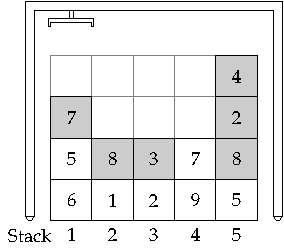
\includegraphics{figs/bay.pdf}
\caption{Container bay.}
\label{fig:bay}
\end{figure}

Let us define the capability of an occupied slot $(s,t)$ by $q(s,t)=p(s,t)$ if the container inside is orderly, otherwise $q(s,t)=0$; specifically, regarding the ground as an occupied slot at tier $0$ with priority value $P$. Thus, we can easily verify the placement of a container $(s,t)$ by checking whether $p(s,t)\le q(s,t-1)$.



The objective of the CPMP is to find an optimized sequence with the fewest container moves capable of converting  the initial layout into a final layout in which all of the containers are orderly.

\section{Generic feasibility-based heuristic scheme}
\label{sec:scheme}

In this section, a generic feasibility-based heuristic scheme is developed for solving the CPMP\@. The proposed heuristic scheme breaks away from the traditional heuristic strategy, contributing to the methodology for the problem. Before describing the heuristic scheme, the concepts of state and state feasibility are introduced first.

\subsection{State and state feasibility}
\label{sec:state}

A state $(\mathsf{L},\boldsymbol{f})$ is a pair comprising a layout $\mathsf{L}$ and a fix vector $\boldsymbol{f}$. The {fix} vector $\boldsymbol{f}$ indicates the fixed height (number of fixed containers) of each stack in $\mathsf{L}$. Further moving of the fixed containers is not allowed. The fixed status of the containers in a layout raises the issue of state feasibility.

\begin{proposition}[Necessary conditions for state feasibility]\label{prop:necessary}
The necessary conditions for the feasibility of a state $(\mathsf{L},\boldsymbol{f})$ are $\boldsymbol{f}\le \boldsymbol{o}$ and $\boldsymbol{\Delta}=\boldsymbol{R}-\boldsymbol{D}\ge \boldsymbol{0}$.
\end{proposition}



Proposition~\ref{prop:necessary} gives the necessary conditions for state feasibility, where $\boldsymbol{R}$ and $\boldsymbol{D}$ are the accumulative resource and demand vectors, and $\boldsymbol{\Delta}$ is the surplus vector. For $1\le p\le P$, $R(p)$ is the order-$p$ accumulative resource described by the total number of slots which can support containers with priority value $p$ (certainly, as well as less than $p$), and $D(p)$ is the order-$p$ accumulative demand or the number of unfixed containers with priority values not less than $p$. Let $d(p)$ be the number of unfixed containers with priority $p$, and $r(p)=\sum_{q^f(s)=p} (H-f(s))$ where $q^f(s)=q(s,f(s))$, we have $D(p)=\sum_{\varphi=p}^P d(\varphi)$ and $R(p)=\sum_{\varphi=p}^P r(\varphi)$. As a result, the non-negativity of the surplus vector $\boldsymbol{\Delta}=\boldsymbol{R}-\boldsymbol{D}$ should be maintained in a feasible state.



For those states where fewer than $S-2$ stacks are fully fixed, the necessary conditions are sufficient to ensure the feasibility of the stack. Taking the layout in Figure~\ref{fig:bay} and $\boldsymbol{f}=\boldsymbol{1}$ as an example, Table~\ref{tab:feasible} illustrates the computation for the surplus vector. The example state is infeasible due to $\Delta(7)<0$; that is, the containers with priority values 7, 8, and 9 cannot be well accommodated by enough unfixed slots.

\begin{table}[htbp]
\caption{Computation for the surplus vector.}
\label{tab:feasible}

\settab

\centering

\begin{tabular*}{\smalltable}{c@{\extracolsep{\fill}}*5{@{}c}}
\toprule
$p$ & $d(p)$ & $D(p)$ & $r(p)$ & $R(p)$ & $\Delta(p)$ \\
\midrule
1 & 0 & 8 & 3 & 15 & 7\\
2 & 1 & 8 & 3 & 12 & 4 \\
3 & 1 & 7 & 0 & 9 & 2\\
4 & 1 & 6 & 0 & 9 & 3\\
5 & 1 & 5 & 3 & 9 & 4 \\
6 & 0 & 4 & 3 & 6 & 2\\
7 & 2 & 4 & 0 & 3 & $-1$\\
8 & 2 & 2 & 0 & 3 & 1\\
9 & 0 & 0 & 3 & 3 & 3\\
\bottomrule
\end{tabular*}

\end{table}


\begin{definition}[Extreme state]
A state $(\mathsf{L},\boldsymbol{f})$ is an extreme state if $|\{s\in\mathbb{S}: f(s)=H\}|\ge S-2$.
\end{definition}



However, in an \emph{extreme} state, i.e., $S-2$ or more stacks are fully fixed, an additional condition is needed. Considering an extreme state, except for $S-2$ fully fixed stacks, if the remaining two stacks cannot be converted into orderly stacks by simply reshuffling unfixed containers from one to the other, we say it is a \emph{tricky} state.

\begin{proposition}[Existence of tricky states]\label{prop:tricky}
A tricky state exists if $E<2(H-1)$.
\end{proposition}




\subsection{Feasibility-based heuristic}

The feasibility-based heuristic first constructs the initial state according to the unreachable tiers. Starting from the initial state, the heuristic repeatedly fixes a target container $c^*$ to a properly chosen slot $(s^-,f(s^-)+1)$, until all of the containers are fixed. The procedure of the heuristic scheme is concisely described in Algorithm~\ref{algo:fbhs}.

\begin{algorithm}[htbp]
\caption{Feasibility-based heuristic scheme.}
\label{algo:fbhs}


\setalgo


\Begin
{
  $(\mathsf{L},\boldsymbol{f})\gets (\mathsf{L}^0,U\cdot\boldsymbol{1})$\;
  \Repeat{$N-SU$}
  {
    $(c^*, s^-)\gets \textrm{the chosen valid task}$\;
    Accomplish $( c^*, s^-) $ on $\mathsf{L}$\;
    $f(s^-)\gets f(s^-)+1$\;
  }
}

\end{algorithm}

\subsection{Initialization}

The initial state is generated with the initial layout $\mathsf{L}^0$ and the initial fix vector $U\cdot\boldsymbol{1}$. It is a natural fact that when $S\ge 3$, the reachable (upper $H-U$) tiers can be permuted into any wanted placement. Meanwhile, the bottom $U$ tiers are unreachable. With the help of the state feasibility concept, we can check the solubility of an instance by checking the feasibility of the initial state.

\begin{proposition}[Instance solubility]
A CPMP instance is solvable if the induced initial state is feasible.
\end{proposition}


\subsection{Valid task}
\label{sec:valid}

At every step of the generic heuristic scheme, a {task} is determined and then accomplished through a sequence of moves. The task is an assignment that aims to fix a chosen target container to the lowest unfixed slot of a chosen aim stack.

A container--stack pair $(c,s)$ is a valid task for the current state $( \mathsf{L},\boldsymbol{f})$ only if (necessary but not sufficient)
\begin{itemize}
\item $c$ is unfixed,
\item $f(s)<H$,
\item $p(c)\le q^f(s)$, and
\item $\Delta(\varphi)\ge H-f(s)$, for $p(c)< \varphi\le q^f(s)$.
\end{itemize}

The last condition ensures the non-negativity of the resulting surplus vector, however, the feasibility of the resulting state is not sufficiently ensured, due to the possibility of tricky state.

There are three methods for resolving the tricky state issue.
\begin{enumerate}
\item Prevent from entering a tricky state when deciding the next task;
\item Design an ideal task accomplishment procedure that makes the resulting extreme state feasible;
\item Allow entering a tricky state and resolve the regression issue.
\end{enumerate}

Our previous work~\citep{wang2015} adopts the last method listed above. The regression issue involves temporarily moving an already fixed container during the task accomplishment, and moving it back to its originally fixed slot.

In Section~\ref{sec:avoid}, we introduce a tricky state avoidance technique that inhibits  the heuristic from entering a tricky state, saving unnecessary moves when solving dense instances.



\section{Available techniques}
\label{sec:technique}
In this section, four available techniques applicable to the feasibility-based heuristic are introduced.

\subsection{Container stability}

Considering an orderly container $(s,t)$ in a feasible state $(\mathsf{L},\boldsymbol{f})$, we say it is \emph{stable} if the revised state $(\mathsf{L},\boldsymbol{f}')$ is feasible such that $f'(s)=t$ and $f'(i)=f(i)$ for $i\neq s$. Denoting the stable height (number of stable containers) of stack $s$ by $ g(s)$, we have $\boldsymbol{f}\le \boldsymbol{ g}\le \boldsymbol{o}\le \boldsymbol{h}$. If the top container of some stack, named $c$ for example, will be stable after being moved to a non-full stack $s$, we say stack $s$ can \emph{stabilize} container $c$.

Figure~\ref{fig:stable} gives an example of a state, where unstable containers are labelled with gray background. Notice that the container $(2,1)$ with priority value $6$ is orderly but unstable.

\begin{figure}[htbp]
\centering
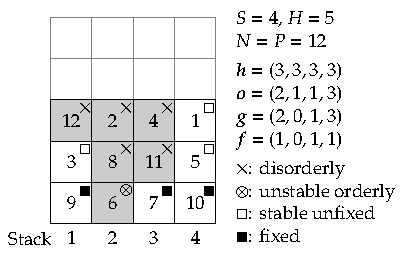
\includegraphics{figs/stable.pdf}
\caption{Stability of containers.}
\label{fig:stable}
\end{figure}

An orderly but unstable container indicates that its orderliness is valueless because it definitely requires reshuffling.
Using the concept of container stability instead of container orderliness is more precise, as an orderly but unstable container has no opportunity to be fixed to its slot.
For example, when a blocking container is becoming orderly but unstable onto a destination stack, the attractiveness of such a move should be reconsidered.






Note that the stability of containers should be recomputed after any container is fixed.


\subsection{Tricky state avoidance}
\label{sec:avoid}

When talking about selecting the next task, the tricky state issue is inevitable. If a container--stack pair leads to an extreme state, the feasibility of the resulting state is unpredictable unless a complicated accomplishment procedure is designed. If unfortunately, a tricky state results, the remainder of the pre-marshalling work must consider the regression issue.

\begin{definition}[Pre-tricky state]\label{def:pre-tricky}
A state is a pre-tricky state if $|\{s\in\mathbb{S}: f(s)=H\}|=S-3$, $|\{s\in\mathbb{S}: f(s)=H-1\}|\ge 1$ and $\sum_{s\in\mathbb{S}}f(s)<N-2$.
\end{definition}


With the introduction of \emph{pre-tricky} state by Definition~\ref{def:pre-tricky}, the tricky state avoidance technique can be summarized as follows. When the current state is pre-tricky, we eliminate the container--stack pairs $(c,s)$ such that $f(s)=H-1$ to avoid entering a tricky state.

\subsection{Bottom tiers protection}

In the feasibility-based heuristic scheme, the target container can be freely chosen as long as the task is valid, not subject to the largest priority value. After the target container $c^*$ is fixed to the aim slot $(s^-,f(s^-)+1)$, the surplus $\Delta(\varphi)$ is reduced by $H-f(s^-)$, for $p(c^*)< \varphi\le q^f(s^-)$.

The bottom tiers protection technique balances the trade-off between the target freedom and the surplus loss, by eliminating the container--stack pairs $(c,s)$ such that $f(s)<2$ and $\delta(p(c),q^f(s))\ge S$, where $\delta(p,q)=\sum_{\varphi=p+1}^{q}d(\varphi)$. The affected demand quantity $\delta(p(c),q^f(s))$ should not reach the threshold $S$ in the bottom two tiers that are protected.

As customizable parameters, the number of tiers protected and the threshold value can be adjusted optionally.

\subsection{Speedy task accomplishment procedure}

\label{sec:speedy}

After the task is decided by specific rules, it is accomplished by a sequence of moves, resulting in a new state. The speedy task accomplishment procedure (STAP) provides a structured framework to finish the given task with the fewest moves, providing customizable interfaces with several user-defined functions.

\subsubsection{Common functions}

The pseudo-code for the common functions of the STAP is given in Algorithm~\ref{algo:common}.

\begin{algorithm*}[htbp]

\caption{Common functions.}
\label{algo:common}
\setalgo


\begin{multicols}{2}

\Procedure{\Move{$\mss,k,\mds$}}
{
  Move $k$ containers from stack $\mss$ to stack $\mds$\;

}

\Procedure{\Relocate{$\mss,k,\mathbb{R}$}}
{
  \Repeat{k}
  {
    $\mathbb{R}'\gets \{s\in \mathbb{R}:h(s)<H\}$\;
    $\mds\gets \arg\min_{s\in\mathbb{R}'} \EvalMove{$\mss,s$}$\;
    \Move{$\mss,1,\mds$}\;
  }
}


\Procedure{\BiSender{$\mss_1,k_1,\mss_2,k_2,\mathbb{R}$}}
{
  $i\gets k_1$, $j\gets k_2$\;
  \Repeat{$k_1+k_2$}
  {
    \uIf{$j=0$}{
      \Relocate{$\mss_1,i,\mathbb{R}$}\;
      $i\gets 0$\;
    }
    \uElseIf{$i=0$}{
      \Relocate{$\mss_2,j,\mathbb{R}$}\;
      $j\gets 0$\;
    }
    \Else
    {
      $\mathbb{R}'\gets \{s\in \mathbb{R}:h(s)<H\}$\;
      $\mds_1\gets \arg\min_{s\in\mathbb{R}'} \EvalMove{$\mss_1,s$}$\;
      $\vec{v}_1\gets \EvalMove{$\mss_1,\mds_1$}$\;
      $\mds_2\gets \arg\min_{s\in\mathbb{R}'} \EvalMove{$\mss_2,s$}$\;
      $\vec{v}_2\gets \EvalMove{$\mss_2,\mds_2$}$\;
      \eIf{$\vec{v}_1\le^{\mathrm{lex}} \vec{v}_2$}
      {
        \Move{$\mss_1,1,\mds_1$}\;
        $i\gets i-1$;
      }
      {
        \Move{$\mss_2,1,\mds_2$}\;
        $j\gets j-1$\;
      }
    }
  }
}
\Function{\MoveNeed{$c,s$}}
{
  \uIf{$(c,s)$ is immediate}
  {
    \Return 0\;
  }
  \Else
  {
    \Return actual number of moves needed by the STAP to accomplish the task $(c,s)$\;
    }
}
\Procedure{\BiReceiver{$\mss,k_1,\mathbb{R}_1,k_2,\mathbb{R}_2$}}
{
  $i\gets k_1$, $j\gets k_2$\;
  \Repeat{$k_1+k_2$}
  {
    \uIf{$j=0$}{
      \Relocate{$\mss,i,\mathbb{R}_1$}\;
      $i\gets 0$\;
    }
    \uElseIf{$i=0$}
    {
      \Relocate{$\mss,j,\mathbb{R}_2$}\;
      $j\gets 0$\;
    }
    \Else
    {
      $\mathbb{R}_1'\gets \{s\in \mathbb{R}_1:h(s)<H\}$\;
      $\mathbb{R}_2'\gets \{s\in \mathbb{R}_2:h(s)<H\}$\;


      $\mds_1\gets \arg\min_{s\in\mathbb{R}_1'} \EvalMove{$\mss,s$}$\;
      $\vec{v}_1\gets \EvalMove{$\mss,\mds_1$}$\;
      $\mds_2\gets \arg\min_{s\in\mathbb{R}_2'} \EvalMove{$\mss,s$}$\;
      $\vec{v}_2\gets \EvalMove{$\mss,\mds_2$}$\;

      \eIf{$\vec{v}_1\le^{\mathrm{lex}}\vec{v}_2$}
      {
        \Move{$\mss,\mds_1$}\;
        $i\gets i-1$\;
      }
      {
        \Move{$\mss,\mds_2$}\;
        $j\gets j-1$\;
      }
    }
  }
}







\end{multicols}

\BlankLine
\BlankLine
\end{algorithm*}


Function \Move{$\mss,k,\mds$} performs $k$ relocations from stack $\mss$ to stack $\mds$.
Function \Relocate{$\mss,k,\mathbb{R}$} performs $k$ relocations from a {sender} stack $\mss$ to a {receiver} set $\mathbb{R}$. For each of the top $k$ containers of the sender, the destination stack $\mds$ is properly selected from $\mathbb{R}$ according to the evaluations by the user-defined function \EvalMove{$\mss,\mds$}. The evaluations of moves are represented by numerical tuples, which are lexicographically comparable.
Function \MoveNeed{$c,s$} returns the actual number of moves performed by the STAP to accomplish the given task $(c,s)$.

Function \BiReceiver{$\mss,k_1,\mathbb{R}_1,k_2,\mathbb{R}_2$} relocates $k_1$ and $k_2$ containers from one sender stack $\mss$ to two receiver sets, $\mathbb{R}_1$ and $\mathbb{R}_2$, respectively. Similarly, function \BiSender{$\mss_1,k_1,\mss_2,k_2,\mathbb{R}$} performs relocations from two senders, stacks $\mss_1$ and $\mss_2$, to the same receiver set $\mathbb{R}$, and the respective quantities are $k_1$ and $k_2$. The moving order of the two top containers from two senders is determined by the smaller evaluation tuple.

\subsubsection{User-defined functions}

User-defined functions in the STAP include
\begin{itemize}
\item  \EvalMove{$\mss,\mds$} returns the penalty of the move from stack $\mss$ to $\mds$;
\item \Interim{$\mathbb{I}$} selects the interim stack from set $\mathbb{I}$; and
\item \InterimFull{$\mathbb{F}$} selects the interim stack from set $\mathbb{F}$, which consists of $S-2$ full stacks.
\end{itemize}



\subsubsection{Task types}


Let the target container be denoted by $c^*(s^+,t^+)$ and the aim stack by $s^-$. The task is \emph{immediate} if it is already located in the aim slot; \emph{internal} if the aim slot is below the target container in the same stack; and \emph{external} if the aim slot is in a different stack.


\subsubsection{Immediate task}

An immediate task does not require a move because the target container is already located in the aim slot; that is, $\MoveNeed{$c^*,s^-$}=0$ for an immediate task $(c^*,s^-)$.

\subsubsection{Internal task}

For an internal task, let $a$ denote the number of empty slots in $\mathbb{S}\setminus\{s^+\}$ with the exclusion of the highest non-full stack; that is, $a=E-e(s^+)-\min\{e(s)>0: s\neq s^+\}$. If multiple stacks are with the maximum height, only one is excluded. Let $b_1$ and $b_2$ denote the numbers of blocking containers above and below $c^*$ in stack $s^+$, respectively. The accomplishment for an internal tack is given in  Algorithm~\ref{algo:internal}, which is divided into three situations:
\begin{itemize}
\item I1: $a\ge b_2$;
\item I2: $a<b_2$ \& $|\{s\neq s^+: h(s)<H\}|>1$; and
\item I3: $a<b_2$ \& $|\{s\neq s^+: h(s)<H\}|=1$.
\end{itemize}


\begin{algorithm*}[htbp]

\caption{Accomplish an internal task.}
\label{algo:internal}

\setalgo

\SetKwProg{One}{case I1:}{}{end~case}
\SetKwProg{Two}{case I2:}{}{end~case}
\SetKwProg{Three}{case I3:}{}{end~case}
\SetKwInput{Target}{target container}
\SetKwInput{Aim}{aim slot}
\SetKwInput{Above}{blocking above}
\SetKwInput{Below}{blocking below}
\SetKwInput{Slot}{slot supply}


\begin{multicols}{2}

\Target{$c^*(s^+,t^+)$}

\Aim{$(s^+,f(s^+)+1)$}
\Slot{$a=E-e(s^+)-\min\{e(s)>0: s\neq s^+\}$}

\Above{$b_1=h(s^+)-t^+$}
\Below{$b_2=t^+-f(s^+)-1$}
\end{multicols}


\begin{multicols}{2}



\Function{$\alpha(s^+,\mds)$}
{
  $e^{\min}\gets \min\{e(s)>0:s\neq s^+\}$\;
  $e^{\sec}\gets \min\{e(s)>e^{\min}:s\neq s^+\}$\;
  $k^{\min}\gets |\{s\neq s^+ : e(s)=e^{\min}\}|$\;
  \uIf{$e(\mds)> e^{\min}$}
  {
    \Return $E-e(s^+)-e^{\min}-1$\;
  }
  \uElseIf{$e^{\min}\ge 2$}
  {
    \Return $E-e(s^+)-e^{\min}$\;
  }
  \uElseIf{$k^{\min}=1$}
  {
     \Return $E-e(s^+)-e^{\sec}-1$\;
  }
  \Else
  {
    \Return $E-e(s^+)-2$\;
  }
}

  \One{$a\ge b_2$}
  {
    \Repeat{$b_1$}
    {

      $\mathbb{R}\gets \{s\neq s^+: h(s)<H,\, \alpha(s^+,s)\ge b_2\}$\;

      \Relocate{$s^+,1,\mathbb{R}$}\;
    }
    $\mathbb{I}\gets \{s\neq s^+: h(s)<H,\, E-e(s^+)-e(s)\ge b_2\}$\;

    $\mts\gets \Interim{$\mathbb{I}$}$\;
    \Move{$s^+,1,s'$}\;
    \Relocate{$s^+,b_2,\mathbb{S}\setminus\{s^+,\mts\}$}\;
    \Move{$\mts,1,s^+$}\;
    \tcp{I1:\ $b_1+b_2+2$ moves}
  }

  \Two{$a<b_2$ \& $|\{s\neq s^+: h(s)<H\}|>1$}
  {
    \Relocate{$s^+, b_1, \mathbb{S}\setminus\{s^+\}$}\;
    $\mts_1\gets \Interim{$\mathbb{S}\setminus\{s^+\}$}$\;
    \Move{$s^+, 1, \mts_1$}\;
    $k_2\gets E-e(s^+)-e(\mts_1)-1$\;
    \Relocate{$s^+, k_2, \mathbb{S}\setminus\{s^+,\mts_1\}$}\;
    Find $\mts_2$ s.t.\ $\mts_2\not\in \{s^+,\mts_1\}$ \& $h(\mts_2)<H$\;
    \Move{$\mts_1, 1, \mts_2$}\;
    \Move{$s^+, b_2-k_2, \mts_1$}\;
    \Move{$\mts_2, 1, s^+$}\;
    \tcp{I2:\ $b_1+b_2+3$ moves}
  }

  \Three{$a<b_2$ \& $|\{s\neq s^+: h(s)<H\}|=1$}
  {
    Find $s'$ s.t.\ $s'\neq s^+$ \& $h(s')<H$\;
    $\mts\gets \InterimFull{$\mathbb{S}\setminus\{s^+,s'\}$}$\;\label{line:wholly}
    \BiSender{$\mts, 1, s^+, b_1, \{s'\}$}\;\label{line:dualsender}
    \Move{$s^+, 1, \mts$}\;
    \Move{$s^+, b_2, s'$}\;
    \Move{$\mts, 1, s^+$}\;
    \tcp{I3:\ $b_1+b_2+3$ moves}
    \tcp{(regression issue not yet included)}
    Resolve regression issue (cf.\ Section~\ref{sec:reg})\;
  }

\end{multicols}
\BlankLine
\BlankLine
\end{algorithm*}

In case I1, a new function $\alpha(s^+,s)$ is defined similar to $a$, representing the number of empty slots in $\mathbb{S}\setminus\{s^+\}$ with the exclusion of the highest non-full stack, after the topmost blocking container of stack $s^+$ is moved to stack $s$. When the blocking containers above the target container are being relocated, the detection of enough slots is performed,  to prevent unnecessary additional moves.

Note that in case I2, the target container $c^*$ is moved to the new interim stack $\mts_2$ from the first interim stack $\mts_1$ when there is only one empty slot remaining in $\mathbb{S}\setminus\{s^+,\mts_1\}$. This can be modified so that $c^*$ can be moved to a new interim stack $\mts_2$ earlier as long as the empty slots in $\mathbb{S}\setminus\{s^+,\mts_2\}$ are enough for the remaining blocking containers in stack $s^+$. Moreover, if there is a full stack in $\mathbb{S}\setminus\{s^+\}$ in case I2, the task can also be completed in a similar way as that used in case I3, with the same operational cost.

\subsubsection{External task}

For an external task, the number of empty slots in $\mathbb{S}\setminus\{s^+,s^-\}$ is denoted by $a$; that is, $a=E-e(s^+)-e(s^-)$. Let $b_1$ and $b_2$ denote the numbers of blocking containers above the target container $c^*$ and the aim slot $(s^-,f(s^-))$, respectively. The pseudo-code describing the accomplishment for an external task is given in Algorithm~\ref{algo:external}, with four situations considered,\begin{itemize}
\item E1: $a\ge b_1+b_2$;
\item E2: $b_1+1\le a<b_1+b_2$;
\item E3: $1\le a<b_1+\min\{1,b_2\}$; and
\item E4: $a=0<b_1+b_2$.
\end{itemize}



\begin{algorithm*}[htbp]
\caption{Accomplish an external task.}
\label{algo:external}

\setalgo

\SetKwProg{One}{case E1:}{}{end~case}
\SetKwProg{Two}{case E2:}{}{end~case}
\SetKwProg{Three}{case E3:}{}{end~case}
\SetKwProg{Four}{case E4:}{}{end~case}
\SetKwInput{Target}{target container}
\SetKwInput{Aim}{aim slot}
\SetKwInput{BPlus}{blocking above target}
\SetKwInput{BMinus}{blocking in aim stack}
\SetKwInput{Slot}{slot supply}


\begin{multicols}{2}

\Target{$c^*(s^+,t^+)$}
\Aim{$(s^-,f(s^-)+1)$}
\BPlus{$b_1=h(s^+)-t^+$}
\BMinus{$b_2=h(s^-)-f(s^-)$}
\Slot{$a=E-e(s^+)-e(s^-)$}

  \One{$a\ge b_1+b_2$}
  {
    \BiSender{$s^+, b_1,s^-,b_2, \mathbb{S}\setminus\{s^+,s^-\}$}\;
    \Move{$s^+, 1, s^-$}\;
    \tcp{E1:\ $b_1+b_2+1$ moves}
  }

  \Two{$b_1+1\le a<b_1+b_2$}
  {
    $k_2\gets a-1-b_1$\;
    \BiSender{$s^+, b_1, s^-, k_2, \mathbb{S}\setminus\{s^+,s^-\}$}\;
    Find $\mts$ s.t.\ $\mts\not\in \{s^+,s^-\}$ \& $h(\mts)<H$\;
    \Move{$s^+,1,\mts$}\;
    \Move{$s^-, b_2-k_2, s^+$}\;
    \Move{$\mts, 1, s^-$}\;
    \tcp{E2:\ $b_1+b_2+2$ moves}
  }


  \Three{$1\le a<b_1+\min\{1,b_2\}$}
  {
    $k_1\gets a-1$\;
    \BiReceiver{$s^+, k_1, \mathbb{S}\setminus\{s^+,s^-\}, b_1-k_1, \{s^-\}$}\;\label{line:dualreceiver}
    Find $\mts$ s.t.\ $\mts\not\in \{s^+,s^-\}$ \& $h(\mts)<H$\;
    \Move{$s^+,1,\mts$}\;
    \Move{$s^-, b_1-k_1+b_2, s^+$}\;
    \Move{$\mts, 1, s^-$}\;
    \tcp{E3:\ $2b_1+b_2-a+3$ moves}
  }

  \Four{$a=0<b_1+b_2$}
  {
    $\mts\gets \InterimFull{$\mathbb{S}\setminus\{s^+,s^-\}$}$\;\label{line:fixed}
    \BiSender{$\mts, 1, s^+, b_1, \{s^-\}$}\;
    \Move{$s^+, 1, \mts$}\;
    \Move{$s^-, b_1+b_2+1, s^+$}\;
    \Move{$\mts, 1, s^-$}\;
    \tcp{E4:\ $2b_1+b_2+4$ moves}
    \tcp{(regression issue not yet included)}
    Resolve regression issue (cf.\ Section~\ref{sec:reg})\;
  }

\end{multicols}

\BlankLine
\BlankLine
\end{algorithm*}



\subsubsection{Regression issue}
\label{sec:reg}

In cases I3 and E4, if the top container of the full stack selected (cf.\ line~\ref{line:wholly} in Algorithm~\ref{algo:internal} and line~\ref{line:fixed} in Algorithm~\ref{algo:external}) is not fixed, the task is done without any side effect. However, if the top container has been fixed, the container should be returned to its previously fixed slot, requiring additional moves.

The regression issue only occurs in tricky states, and it can be avoided if the tricky state avoidance technique (cf.\ Section~\ref{sec:avoid}) is applied.



\section{Greedy and speedy heuristic}

\label{sec:gash}


The proposed {greedy and speedy heuristic} (GASH) is a realized implementation of the generic feasibility-based heuristic scheme.
The GASH employs all the techniques introduced above, i.e., the container stability concept, the techniques of tricky state avoidance and bottom tiers protection, and the STAP\@. The procedure of the GASH and the user-defined functions for the STAP are given in Algorithm~\ref{algo:gash}.



\begin{algorithm*}[htbp]
\caption{Greedy and speedy heuristic.}
\label{algo:gash}


\setalgo


\begin{multicols}{2}
\Begin
{
  $(\mathsf{L},\boldsymbol{f})\gets (\mathsf{L}^0,U\cdot\boldsymbol{1})$\;
  \Repeat{$N-SU$}
  {
    $\mathbb{T}\gets \Valid{}$\;
    $(c^*, s^-)\gets \arg\min_{(c,s)\in\mathbb{T}} \EvalTask{$c,s$}$\;
    Accomplish $( c^*, s^-)$ by the STAP\;
    $f(s^-)\gets f(s^-)+1$\;
  }
}

\Function{\Valid{}}
{
  $\mathbb{T}\gets \varnothing$\;

  \ForEach{$(c,s)\in\mathbb{C}\times\mathbb{S}$}
  {
      \If{$c$ is unfixed \\\& $f(s)<H$ \\\& $p(c)\le q^f(s)$ \\\& $\Delta(\varphi)\ge H-f(s)$, for $p(c)< \varphi\le q^f(s)$}
      {
        $\mathbb{T}\gets \mathbb{T}\cup\{(c,s)\}$\;
      }
  }
  \Return $\mathbb{T}$\;
}



\Function{\EvalTask{$c,s$}}
{
  $p\gets p(c)$\;
  $q\gets q^f(s,f(s))$\;
  $\chi\gets 0$ \tcp*[l]{key indicator}
  \If{$f(s)<2$ \& $\delta(p,q)\ge S$}
  {
    \tcp{bottom tiers protection}
    $\chi\gets \infty$\;
  }
  \If{$(\mathsf{L},\boldsymbol{f})$ is pre-tricky \& $f(s)=H-1$}
  {
    \tcp{tricky state avoidance}
    $\chi\gets \infty$\;
  }

  $n\gets \MoveNeed{$c,s$}$\;

  \Return $\langle \chi,\ n,\  g(s)-f(s),\ \delta(p,q),\ f(s),\ -p(c) \rangle$\;
}



\Function{\EvalMove{$\mss,\mds$}}
{
  $c\gets (\mss,h(\mss))$\;
  $p\gets p(c)$\;
  $q\gets q(\mds,h(\mds))$\;
  \uCase{$ g(\mds)=h(\mds)$ \& stack $\mds$ can stabilize $c$}
  {
    \Return $\langle 1,\ \delta(p,q) \rangle$\;
  }
  \uCase{$ g(\mds)<h(\mds)$ \& $p\ge m(\mds)$}
  {
    \Return $\langle 2,\ p-m(\mds) \rangle$\;
  }
  \uCase{$ g(\mds)<h(\mds)$ \& $p<m(\mds)$}
  {
    \Return $\langle 3,\ m(\mds)-p \rangle$\;
  }
  \Case{$ g(\mds)=h(\mds)$ \& stack $s_2$ cannot stabilize $c$}
  {
    \Return $\langle 4,\ q \rangle$\;
  }
}



\Function{\Interim{$\mathbb{I}$}}
{
  $\mathbb{I}_1\gets \{s\in \mathbb{I}:  g(s)<h(s)<H\}$\;
  $\mathbb{I}_2\gets \{s\in \mathbb{I}:  g(s)=h(s)<H\}$\;

  \uIf{$\mathbb{I}_1\neq \varnothing$}
  {
    \Return $\arg\max_{s\in\mathbb{I}_1} m(s)$\;
  }
  \Else
  {
    \Return $\arg\min_{s\in\mathbb{I}_2} q(s,h(s))$\;
  }

}




\Function{\InterimFull{$\mathbb{F}$}}
{
  $\mathbb{F}_1\gets \{s\in \mathbb{F}: f(s)\le g(s)<h(s)=H\}$\;
  $\mathbb{F}_2\gets \{s\in \mathbb{F}: f(s)< g(s)=h(s)=H\}$\;
  $\mathbb{F}_3\gets \{s\in \mathbb{F}: f(s)= g(s)=h(s)=H\}$\;
  \uIf{$\mathbb{F}_1\neq \varnothing$}
  {
    \Return $\arg\min_{s\in\mathbb{F}_1} p(s,h(s))$\;
  }
  \uElseIf{$\mathbb{F}_2\neq \varnothing$}
  {
    \Return $\arg\min_{s\in\mathbb{F}_2} p(s,h(s))$\;
  }
  \Else(\tcp*[h]{cause regression issue})
  {
    \Return $\arg\min_{s\in\mathbb{F}_3} p(s,h(s))$\;
  }
}

\end{multicols}
\BlankLine
\BlankLine
\end{algorithm*}



Function \Valid{} returns $\mathbb{T}$, the set of valid tasks for the current state. Every task $(c,s)\in\mathbb{T}$ is then evaluated by function \EvalTask{$c,s$}. The evaluation of a container--stack pair $(c,s)$ is a six-tuple, that starts with the key indicator, followed by the actual number of moves required by the STAP, the number of  stable containers that need to be moved from the aim stack, the affected demand, fixed height of the aim stack, and the opposite of the target container's priority value. At every step of the GASH, the next task is determined by the lexicographically minimum evaluation six-tuple.


Define the \emph{messiness} of stack $s$ by $m(s)=\max_{g(s)<t\le h(s)}p(s,t)$, that is the largest priority value among the unstable containers in stack $s$. The preferences of selecting a stack $\mds$ as the destination stack for a blocking container are as follows.
\begin{enumerate}
\item If stack $\mds$ is entirely stable and can stabilize $c$, the minimum affected demand is preferred;
\item If stack $\mds$ is not entirely stable and $p(c)\ge m(\mds)$, the minimum gap between $m(\mds)$ and $p(c)$ is preferred;
\item If stack $\mds$ is not entirely stable and $p(c)> m(\mds)$, the minimum gap between $p(c)$ and $m(\mds)$ is preferred;
\item If stack $\mds$ is entirely stable but cannot stabilize $c$, the minimum $q(\mds,h(\mds))$ is preferred.
\end{enumerate}

The first preference indicates that stabilizing a blocking container reduces the total number of unstable containers in the bay. The second and third preferences consider the messiness of the destination stack. Messiness refers to the largest priority value of the unstable containers in a stack; larger messiness implies a higher urgency of reshuffling. The last preference indicates that an entirely stable stack should be protected from being ruined.

In cases I1 and I2, an interim stack is selected to temporarily store the target container.
The selection prefers stacks that are not entirely stable, with the largest messiness, then entirely stable stacks with the smallest capability. The most unattractive stack for receiving blocking containers is selected as the interim stack. In cases I3 and E4, the interim stack is selected by the minimum priority value of the top containers of these full stacks.

Note that because the tricky state avoidance technique is applied, the regression issue would never happen in the GASH, although it is still considered in function \InterimFull{$\mathbb{F}$} to complete the whole logic.

\section{Computational results}
\label{sec:experiment}

In this section, the proposed greedy and speedy heuristic (GASH) is compared to two benchmark heuristic approaches. One is the target-guided heuristic (TGH) proposed in our previous work \citep{wang2015}, and the other is a similar implementation to the LPFH proposed by \cite{exp2012}. Since the LPFH only discusses cases with enough empty slots (cases I1 and E1 in our statement) and involves random decisions, it is difficult to implement a deterministic version. Thus, we develop a substitute instead, referred to as the largest priority value first heuristic (LPVFH).

The LPVFH selects the next target container from unfixed containers with the largest priority value, and then accomplish it by the STAP with the same user-defined functions used as that in the GASH\@. Necessary pseudo-code for the LPVFH is given in Algorithm~\ref{algo:lpvfh}.

\begin{algorithm*}[htbp]
\caption{Largest priority value first heuristic.}
\label{algo:lpvfh}


\setalgo

\begin{multicols}{2}

\Begin
{
  $(\mathsf{L},\boldsymbol{f})\gets (\mathsf{L}^0,U\cdot\boldsymbol{1})$\;

  \ForEach{$p=P,\dots,1$}
  {
    $\mathbb{C}_p\gets\textrm{containers with priority value $p$}$\;
    $\mathbb{A}_p\gets\varnothing$\tcp*[l]{set of aim stacks}
    \While{$\mathbb{C}_p\neq \varnothing$}
    {
      $(c^*, s^-)\gets \arg\min_{c\in\mathbb{C}_p, f(s)<H} \MoveNeed{$c,s$}$\;
      Accomplish $( c^*, s^-)$ by the STAP\;
      $f(s^-)\gets f(s^-)+1$\;
      $\mathbb{C}_p\gets\mathbb{C}_p\setminus\{c^*\}$\;
      $\mathbb{A}_p\gets \mathbb{A}_p\cup \{s^-\}$\;
    }
    \ForEach{$s^-\in\mathbb{A}_p$}
    {
    	\Fill{$s^-$}\;
    }
  }
}



\Function{\Fill{$s^-$}}
{
  \While{$h(s^-)<H$}
  {
    $\mathbb{S}'\gets\varnothing$\;
    \ForEach{$s\in\{s\neq s^-: g(s)<h(s)\}$}
    {
      $c\gets (s,h(s))$\;
      \If{ stack $s^-$ can stabilize $c$}
      {
        $\mathbb{S}'\gets \mathbb{S}'\cup \{s\}$\;
      }
    }
    \eIf{$\mathbb{S}'\neq \varnothing$}
    {
      $s'\gets \arg\max_{s\in\mathbb{S}'} p(s,h(s))$\;
      \Move{$s',1,s^-$}\;
    }
    {
      \Break\;
    }
  }
}
\end{multicols}
\BlankLine
\BlankLine
\end{algorithm*}





The problem instance format of the CPMP is the same as that of the {container relocation problem} (CRP, a.k.a.\ the blocks relocation problem), the problem of minimizing the total number of container moves for retrieving containers from the initial layout.
In the literature, researchers usually use the same data sets when solving the CPMP~\citep{bort2012,cas2009,exp2012,wang2015} and the CRP~\citep{cas2011,exp2014,forster2012,jin2013,jin2015}.

\subsection{Results for CVS instances}

\citet{cas2011} present the complete CVS data set (named after the authors' surnames, Caserta, Vo{\ss} and Sniedovich) originally for the CRP\@. The CVS instances are classified into 21 groups, each consisting of 40 instances. The stacks of the initial layout have the same height in a CVS instance. The number of containers per stack in the initial layout is denoted by $K$, hence $N=SK$. It is worth noting that the stack height limitation is not specified in the original data. The researchers add two extra tiers above the initial layout; that is, $H=K+2$.

The CVS instances can be considered typical dense CPMP instances. Table~\ref{tab:cvs} illustrates the computational results on CVS instances by the GASH, the TGH, and the LPVFH\@. The values under the ``move'' headings represent average number of moves for every CVS group, whereas the values under the ``gap\%'' headings are the ratios of the difference between each benchmark heuristic and the GASH to the number of containers $N$. The results showcase that the GASH leads the benchmark heuristics by more than $10\%\times N$ moves on most instance groups. Especially on the narrowest group CVS~10-6, the GASH outperforms the TGH and the LPVFH by 319.38\% and 55.54\%, respectively.

\begin{table}[htbp]
\caption{Results for CVS instances.}
\label{tab:cvs}

\settab

\centering



\begin{tabular*}{\smalltable}{l@{\extracolsep{\fill}}@{}r@{}r@{}r@{}r@{}r}
\toprule
\multirow{2}{*}[-.5\defaultaddspace]{CVS~K-S}&

\multirow{2}{*}[-.5\defaultaddspace]{\begin{tabular}{@{}c@{}}GASH\\move\end{tabular}}&
\multicolumn{2}{@{}c@{}}{TGH}&\multicolumn{2}{@{}c}{LPVFH} \\

\cmidrule{3-4}
\cmidrule(r){5-6}
&   & move & gap\%    & move & gap\%   \\
\midrule
CVS 3-3   &11.28  & 12.95  & 18.61     & 11.25  & $-0.28$     \\
CVS 3-4   &  10.80  & 12.18  & 11.46     & 12.23  & 11.88     \\
CVS 3-5   & 12.08  & 12.78  & 4.67      & 13.45  & 9.17      \\
CVS 3-6   &  12.98  & 14.38  & 7.78      & 14.88  & 10.56     \\
CVS 3-7   & 14.75  & 16.00  & 5.95      & 16.58  & 8.69      \\
CVS 3-8   & 15.65  & 16.55  & 3.75      & 17.08  & 5.94      \\
CVS 4-4   & 21.88  & 23.35  & 9.22      & 21.93  & 0.31      \\
CVS 4-5   &  23.08  & 26.73  & 18.25     & 26.48  & 17.00     \\
CVS 4-6   & 24.75  & 27.58  & 11.77     & 27.20  & 10.21     \\
CVS 4-7   &  27.63  & 29.93  & 8.21      & 31.23  & 12.86     \\
CVS 5-4   & 35.08  & 44.83  & 48.75     & 35.83  & 3.75      \\
CVS 5-5   &  35.33  & 42.40  & 28.30     & 36.50  & 4.70      \\
CVS 5-6   &  39.88  & 50.63  & 35.83     & 43.08  & 10.67     \\
CVS 5-7   &  41.68  & 48.83  & 20.43     & 46.95  & 15.07     \\
CVS 5-8   &  47.50  & 56.68  & 22.94     & 51.83  & 10.81     \\
CVS 5-9   &  50.45  & 57.50  & 15.67     & 55.65  & 11.56     \\
CVS 5-10  & 54.63  & 62.80  & 16.35     & 60.88  & 12.50     \\
CVS 6-6   &  55.23  & 74.33  & 53.06     & 57.85  & 7.29      \\
CVS 6-10  & 75.60  & 88.63  & 21.71     & 79.73  & 6.88      \\
CVS 10-6  & 140.63 & 332.25 & 319.38    & 173.95 & 55.54     \\
CVS 10-10 & 179.23 & 302.90 & 123.68    & 190.50 & 11.28     \\[\defaultaddspace]
Average      & 44.29  & 64.48  & 38.37     & 48.81  & 11.26     \\
\bottomrule
\end{tabular*}
\end{table}

\subsection{Results for BF instances}

\citet{bort2012} introduce 32 groups of CPMP instances (referred to as BF instances), each group consisting of 20 instances. In BF instances, the bay size is $S=16$ or $20$ and $H=5$ or $8$. The number of containers $N$ is either $0.6\times SH$ or $0.8\times SH$, the number of priorities $P$ is either $0.2\times N$ or $0.4\times N$, and the number of disorderly containers  $B$ is either $0.6\times N$ or $0.75\times N$ in the initial layout.

The BF instances can be considered typical loose CPMP instances. Table~\ref{tab:bf} illustrates the computational results on BF instances by the three heuristics. The values under the ``ratio\%'' headings are the relative gap between per heuristic and the number of disorderly containers initially $B$, and the values under the ``gap\%'' headings are the differences between the ``ratio\%'' columns of the GASH and each benchmark heuristic.


\begin{table*}[htbp]
\caption{Results for BF instances.}
\label{tab:bf}

\settab

\centering

\begin{tabular*}{\linewidth}{c@{\extracolsep{\fill}}*5{@{}c}@{}r@{}r@{}r@{}r@{}r@{}r@{}r@{}r}
\toprule
\multirow{2}{*}[-.5\defaultaddspace]{BF}&
\multirow{2}{*}[-.5\defaultaddspace]{S}   &
\multirow{2}{*}[-.5\defaultaddspace]{H}    &
\multirow{2}{*}[-.5\defaultaddspace]{N}   &
\multirow{2}{*}[-.5\defaultaddspace]{P}    &
\multirow{2}{*}[-.5\defaultaddspace]{B}   &
\multicolumn{2}{@{}c@{}}{GASH} & \multicolumn{3}{@{}c@{}}{TGH} &\multicolumn{3}{@{}c}{LPVFH} \\
\cmidrule{7-8}
\cmidrule{9-11}
\cmidrule(r){12-14}
       &  & &   &  &   & move & ratio\% &move & ratio\% & gap\%&move & ratio\% & gap\%\\
\midrule
1  & 16 & 5 & 48  & 10 & 29 & 29.15  & 0.52  & 29.10  & 0.34  & $-0.17$ & 29.55  & 1.90  & 1.38  \\
2  & 16 & 5 & 48  & 10 & 36 & 36.00  & 0.00  & 36.00  & 0.00  & 0.00  & 36.60  & 1.67  & 1.67  \\
3  & 16 & 5 & 48  & 20 & 29 & 29.35  & 1.21  & 29.45  & 1.55  & 0.34  & 30.90  & 6.55  & 5.34  \\
4  & 16 & 5 & 48  & 20 & 36 & 36.15  & 0.42  & 36.00  & 0.00  & $-0.42$ & 37.20  & 3.33  & 2.92  \\
5  & 16 & 5 & 64  & 13 & 39 & 46.30  & 18.72 & 48.50  & 24.36 & 5.64  & 53.00  & 35.90 & 17.18 \\
6  & 16 & 5 & 64  & 13 & 48 & 55.50  & 15.63 & 57.55  & 19.90 & 4.27  & 62.85  & 30.94 & 15.31 \\
7  & 16 & 5 & 64  & 26 & 39 & 49.95  & 28.08 & 53.55  & 37.31 & 9.23  & 57.15  & 46.54 & 18.46 \\
8  & 16 & 5 & 64  & 26 & 48 & 57.60  & 20.00 & 60.00  & 25.00 & 5.00  & 66.90  & 39.38 & 19.38 \\
9  & 16 & 8 & 77  & 16 & 47 & 56.30  & 19.79 & 60.35  & 28.40 & 8.62  & 62.15  & 32.23 & 12.45 \\
10 & 16 & 8 & 77  & 16 & 58 & 61.55  & 6.12  & 62.15  & 7.16  & 1.03  & 69.50  & 19.83 & 13.71 \\
11 & 16 & 8 & 77  & 31 & 47 & 55.00  & 17.02 & 61.25  & 30.32 & 13.30 & 63.70  & 35.53 & 18.51 \\
12 & 16 & 8 & 77  & 31 & 58 & 61.45  & 5.95  & 63.45  & 9.40  & 3.45  & 68.50  & 18.10 & 12.16 \\
13 & 16 & 8 & 103 & 21 & 62 & 96.50  & 55.65 & 107.45 & 73.31 & 17.66 & 110.85 & 78.79 & 23.15 \\
14 & 16 & 8 & 103 & 21 & 78 & 116.05 & 48.78 & 124.75 & 59.94 & 11.15 & 134.90 & 72.95 & 24.17 \\
15 & 16 & 8 & 103 & 42 & 62 & 99.45  & 60.40 & 110.60 & 78.39 & 17.98 & 110.40 & 78.06 & 17.66 \\
16 & 16 & 8 & 103 & 42 & 78 & 115.45 & 48.01 & 133.35 & 70.96 & 22.95 & 137.40 & 76.15 & 28.14 \\
17 & 20 & 5 & 60  & 12 & 36 & 36.50  & 1.39  & 36.50  & 1.39  & 0.00  & 37.35  & 3.75  & 2.36  \\
18 & 20 & 5 & 60  & 12 & 45 & 45.20  & 0.44  & 45.00  & 0.00  & $-0.44$ & 45.00  & 0.00  & -0.44 \\
19 & 20 & 5 & 60  & 24 & 36 & 36.75  & 2.08  & 36.80  & 2.22  & 0.14  & 38.50  & 6.94  & 4.86  \\
20 & 20 & 5 & 60  & 24 & 45 & 45.10  & 0.22  & 45.00  & 0.00  & $-0.22$ & 45.70  & 1.56  & 1.33  \\
21 & 20 & 5 & 80  & 16 & 48 & 56.55  & 17.81 & 61.65  & 28.44 & 10.63 & 65.65  & 36.77 & 18.96 \\
22 & 20 & 5 & 80  & 16 & 60 & 65.55  & 9.25  & 67.90  & 13.17 & 3.92  & 74.50  & 24.17 & 14.92 \\
23 & 20 & 5 & 80  & 32 & 48 & 55.25  & 15.10 & 61.10  & 27.29 & 12.19 & 65.75  & 36.98 & 21.88 \\
24 & 20 & 5 & 80  & 32 & 60 & 68.00  & 13.33 & 70.95  & 18.25 & 4.92  & 76.65  & 27.75 & 14.42 \\
25 & 20 & 8 & 96  & 20 & 58 & 66.00  & 13.79 & 69.80  & 20.34 & 6.55  & 73.60  & 26.90 & 13.10 \\
26 & 20 & 8 & 96  & 20 & 72 & 75.75  & 5.21  & 74.35  & 3.26  & $-1.94$ & 81.75  & 13.54 & 8.33  \\
27 & 20 & 8 & 96  & 39 & 58 & 65.65  & 13.19 & 71.85  & 23.88 & 10.69 & 73.65  & 26.98 & 13.79 \\
28 & 20 & 8 & 96  & 39 & 72 & 76.50  & 6.25  & 76.30  & 5.97  & $-0.28$ & 83.55  & 16.04 & 9.79  \\
29 & 20 & 8 & 128 & 26 & 77 & 115.85 & 50.45 & 118.65 & 54.09 & 3.64  & 128.65 & 67.08 & 16.62 \\
30 & 20 & 8 & 128 & 26 & 96 & 129.60 & 35.00 & 143.05 & 49.01 & 14.01 & 155.15 & 61.61 & 26.61 \\
31 & 20 & 8 & 128 & 52 & 77 & 115.85 & 50.45 & 128.15 & 66.43 & 15.97 & 128.80 & 67.27 & 16.82 \\
32 & 20 & 8 & 128 & 52 & 96 & 134.10 & 39.69 & 147.30 & 53.44 & 13.75 & 157.00 & 63.54 & 23.85\\[\defaultaddspace]
\multicolumn{6}{l@{}}{Average}  & 68.44  & 19.37 & 72.75  & 26.05 & 6.67  & 76.96 &	33.09 &	13.71 \\

\bottomrule


\end{tabular*}

\end{table*}


The relative gap between the solution value and the number of disorderly containers in the initial layout is a good measure of the heuristic performance. Table~\ref{tab:bfsum} shows that the instance density $N/SH$ (or bay utilization) and the height of the bay $H$ are key factors in the number of moves needed for pre-marshalling. In other words, denser or higher instances are more difficult to solve. The computational results on BF instances also prove that the GASH outperforms these two benchmark heuristics.



\begin{table}[htbp]
\caption{Summary on BF instances.}
\label{tab:bfsum}

\settab

\centering

\begin{tabular*}{\smalltable}{c@{\extracolsep{\fill}}r@{}*5{@{}r}}
\toprule

&\multicolumn{2}{@{}c@{}}{GASH} & \multicolumn{2}{@{}c@{}}{TGH} & \multicolumn{2}{@{}c}{LPVFH}\\
&\multicolumn{2}{@{}c@{}}{ratio\%} & \multicolumn{2}{@{}c@{}}{gap\%} & \multicolumn{2}{@{}c}{gap\%}\\
\cmidrule{2-3}\cmidrule{4-5}\cmidrule(r){6-7}
density & $H=5$ & \multicolumn{1}{@{}c@{}}{8} &\multicolumn{1}{@{}c@{}}{5} & \multicolumn{1}{@{}c@{}}{8} & \multicolumn{1}{@{}c@{}}{5} & \multicolumn{1}{@{}c}{8} \\
\midrule
0.6&  0.78  & 10.91  & $-0.10$  & 5.18  & 4.85  & 10.50 \\
0.8&  17.24  & 48.55  & 6.97  & 14.64  & 19.65  & 14.81 \\
\bottomrule
\end{tabular*}

\end{table}



\section{Conclusions}
\label{sec:conclusion}

In this paper we present a generic heuristic scheme based on new concepts of state and state feasibility for solving the container pre-marshalling problem. The proposed heuristic scheme is an innovative departure from the traditional heuristic strategy. Furthermore, a realized instance of the heuristic scheme, the greedy and speedy heuristic, is also proposed. Numerical experiments on two commonly used data sets are conducted, comparing the proposed feasibility-based heuristic to two benchmark heuristics.

A major challenge raised in the feasibility-based heuristic scheme is the trade-off between the freedom of selecting target containers and the waste of the resource surplus. In this paper, the bottom tiers protection technique is proposed to balance the trade-off. As a future work, efforts in better solving the difficulty can be considered to improve the performance of the feasibility-based heuristic. Moreover, new feasibility-based heuristics and meta-heuristics are also worthy exploring.


\section*{References}

%\bibliographystyle{myapa}
\bibliographystyle{apalike2}
\bibliography{cpmp}

\end{document}











